\documentclass[12pt]{article}
\usepackage{fontspec}\setmainfont{Liberation Serif} % Overleaf: chọn XeLaTeX
\usepackage[a4paper,margin=2cm]{geometry}
\usepackage{lhtl-cauhoi}
\begin{document}

\begin{cauhoi}[id=T12-C1-001, loai=mcq, lop=12, chuong=ung-dung-dao-ham, chuyende=don-dieu, mucdo=2, nguon=Tự soạn]
Hàm số $y=x^3-3x+2$ nghịch biến trên khoảng nào dưới đây?
\phuongan
\pa{$(-\infty;-1)$}
\pa*{$(-1;1)$}
\pa{$(1;+\infty)$}
\pa{$(-\infty;+\infty)$}
\loigiai Ta có $y'=3x^2-3$, $y'<0 \Leftrightarrow -1<x<1$. Bảng biến thiên:
\begin{hinh}
\begin{tikzpicture}
\tkzTabInit[lgt=1.5,espcl=2.5]{$x$/0.8,$y'$/0.8,$y$/2}{$-\infty$,$-1$,$1$,$+\infty$}
\tkzTabLine{,+,0,-,0,+,}
\tkzTabVar{-/$-\infty$,+/$4$,-/$0$,+/$+\infty$}
\end{tikzpicture}
\end{hinh}
\end{cauhoi}

\begin{cauhoi}[id=T12-C1-002, loai=true_false, lop=12, chuong=ung-dung-dao-ham, chuyende=cuc-tri, mucdo=2, nguon=Tự soạn]
Cho hàm số $f(x)=x^3-3x+2$. Xét tính đúng sai của các mệnh đề sau:
\cacy
\ydung{$f'(x)=3x^2-3$.}
\ysai{Hàm số đạt cực đại tại $x=1$.}
\ydung{Giá trị cực tiểu của hàm số bằng $0$.}
\ysai{Đồ thị hàm số cắt trục hoành tại ba điểm phân biệt.}
\loigiai $f'(x)=0\Leftrightarrow x=\pm1$; cực đại tại $x=-1$, $f(-1)=4$; cực tiểu tại $x=1$, $f(1)=0$. Vì $f(x)=(x-1)^2(x+2)$ nên đồ thị chỉ có 2 điểm chung với trục hoành.
\end{cauhoi}

\begin{cauhoi}[id=T12-C4-003, loai=short_answer, lop=12, chuong=nguyen-ham-tich-phan, chuyende=tich-phan, mucdo=2, nguon=Tự soạn]
Tính $I=\displaystyle\int_0^1 (2x-1)\,\mathrm{d}x - \dfrac{1}{2}$.
\dapso{-0,5}{-1/2}
\loigiai $\displaystyle\int_0^1(2x-1)\,\mathrm{d}x=\left.(x^2-x)\right|_0^1=0$, nên $I=-\dfrac12=-0{,}5$.
\end{cauhoi}

\begin{cauhoi}[id=T10-C3-004, loai=essay, lop=10, chuong=ham-so-bac-hai, chuyende=do-thi, mucdo=3, nguon=Tự soạn]
Cho hàm số $y=x^2-2x-3$.
a) Lập bảng biến thiên của hàm số.
b) Tìm $m$ để phương trình $x^2-2x-3=m$ có hai nghiệm phân biệt.
\thangdiem{a}{0,5}{Tính đúng đỉnh $I(1;-4)$ (0,25); bảng biến thiên đúng (0,25).}
\thangdiem{b}{0,5}{Lập luận qua đồ thị/bảng biến thiên (0,25); kết luận $m>-4$ (0,25).}
\loigiai a) Đỉnh $I(1;-4)$, hàm số nghịch biến trên $(-\infty;1)$, đồng biến trên $(1;+\infty)$. b) $m>-4$.
\end{cauhoi}

\end{document}
